
\chapter{Wyniki działania algorytmu na popularnych zbiorach danych}

\section{Metodologia pomiarów}
	Żeby oszacować trafność klasyfikacji osiąganą przez skonstruowany system konieczne było podzielenie zbioru danych na zbiór uczący i \emph{testujący}, a w przypadku algorytmu Kernel-GP również wydzielenie ze zbioru uczącego podzbioru \emph{walidującego}, używanego do obliczania miary przystosowania (fitness) podczas przebiegu algorytmu genetycznego. Ponieważ sposób podziału zbioru danych ma wpływ na osiąganą trafność klasyfikacji, dokonywano 5 takich podziałów a następnie wyciągano średnią oraz odchylenie standardowe z wyników otrzymanych dla tych podziałów. Ta procedura dotyczyła zarówno testowania algorytmu \emph{Kernel-GP} jak i porównawczych testów klasyfikatora SVM z biblioteki \emph{LibSVM}. Dla obu algorytmów stosowano te same podziały danych, przy czym w przypadku klasyfikatora \emph{LibSVM} ze zbioru uczącego nie wydzielano zbioru testującego.
	
	Algorytm genetyczny jest w swej naturze stochastyczny, korzysta więc z funkcji generujących liczby pseudolosowe. Aby zapewnić powtarzalność wyników i umożliwić ich porównanie ziarno generatora liczb pseudolosowych ustawiono na stałą wartość.

	Aby ocenić skuteczność algorytmu genetycznego w poszukiwaniu optymalnych funkcji jądrowych oraz oszacować optymalną wielkość populacji, liczbę ewaluowanych pokoleń oraz najlepszą funkcję przystosowania przeprowadzono szereg eksperymentów obliczeniowych, w których uruchamiano algorytm dla coraz to większych wartości tych parametrów. Dla każdego przebiegu algorytmu obliczano i zapisywano kilka miar trafność klasyfikacji zbioru \emph{walidującego} (miary te zostały opisane w części \ref{sec:measures}).

	Analizując tak zebrane dane można przeanalizować na ile poszukiwanie funkcji jądrowej przez algorytm genetyczny było podobne do losowego przeszukiwania a na ile było ono zbieżne. W pierwszym przypadku na wyniki osiągane przez algorytm powinna mieć wpływ przede wszystkim wielkość populacji, w drugim również liczba populacji przez które poszukiwano rozwiązania. W szczególności ciekawym przypadkiem jest ten, gdy liczba populacji wynosi 1, czyli cały algorytm ogranicza się do wygenerowania populacji losowych osobników i wybrania jednego z nich - w tym przypadku algorytm genetyczny sprowadza się do losowego poszukiwania rozwiązania. Porównując różnicę w trafności osiąganej w trakcie jednego pokolenia i coraz większej ich liczby można ocenić czy proces ewolucyjny przebiega poprawnie.
	
\section{Parametry algorytmu}
Tabela \ref{tab:params-gp} przedstawia użyte w eksperymentach wartości parametrów procesu ewolucyjnego.
\begin{table}
	\caption{Parametry procesu ewolucyjnego \label{tab:params-gp}}
	\begin{tabular}{|r||c|c|}
	\hline
	• & mimimum & maksimum \\ 
	\hline \hline 
	Wielkość populacji & 1 & 100 \\ 
	\hline
	Liczba pokoleń & 1 & 50 \\ 
	\hline 
	Głębokość generowanych drzew & 3 & 8 \\ 
	\hline 
	Prawdopodobieństwo mutacji & - & 0.55 \\ 
	\hline 
	Prawdopodobieństwo krzyżowania & - & 0.4 \\ 
	\hline 
	Prawdopodobieństwo klonowania & - & 0.05 \\ 
	\hline 
	Prawdopodobieństwo mutacji stałych & - & 0.9 \\ 
	\hline 
	Wielkość turnieju & • & 7 \\ 
	\hline 
	Ilość koszyków  & • & 10 \\ 
	\hline 
	\end{tabular} 
\end{table}
	
\section{Opis zbiorów danych}
	Do oceny pracy algorytmu użyto standardowych zbiorów danych służących do testowania systemów maszynowego uczenia się, dostępnych na stronie biblioteki \emph{LIBSVM} \cite{chang_libsvm:_2011}  oraz w repozytorium UCI \cite{Bache+Lichman:2013} [\ref{url:uci}]. Zbiory zostały opisane w tabelce \ref{tab:datasets}. Użyte nazwy zbiorów są zgodne z tymi ze strony libsvm [\ref{url:libsvm}].

\newcolumntype{Z}{>{\centering\arraybackslash}m{17mm}}

\begin{table}[ht]
	\caption{Zbiory danych użyte do testowania systemu.\label{tab:datasets}} 	
%	\begin{tabular}{|p{2cm}||r|p{1.5cm}|p{1.5cm}|p{1.5cm}|p{1.5cm}|p{1.5cm}|}
	\begin{tabulary}{1.0\textwidth}{|r||r|r|r|r|r|r|}
		\hline 
		\multicolumn{1}{|Z||}{Nazwa zbioru}   & \multicolumn{1}{Z|}{Liczba klas}  & \multicolumn{1}{Z|}{ Liczba atrybutów}  & \multicolumn{1}{Z|}{ Wielkość zbioru}  & \multicolumn{1}{Z|}{ Wielkość zbioru uczącego}  & \multicolumn{1}{Z|}{Wielkość zbioru testującego}  & \multicolumn{1}{Z|}{Wielkość zbioru walidującego} \\
		\hline \hline
		Iris & 3 & 4 & 150 & 68 & 33 & 49  \\ 
		\hline 
		Letter & 26 & 16 & 15000 & 9000 & 4400 & 6600\\ 
		\hline 
		DNA & 3 & 180 & 2000 & 1435 & 700 & 1051 \\ 
		\hline 
		Vowel & 11 & 10 & 528 & 447 & 217 & 326 \\ 
		\hline
		Breast cancer & 2 & 10 & 683 & 409 & 274 & 33.00\% \\ \hline
		Heart (statlog)& 2 & 13 & 270 & 180 & 90 & 33.00\% \\ \hline
		Ionosphere & 2 & 34 & 351 & 234 & 117 & 33.00\% \\ \hline
		Liver disorders & 2 & 6 & 345 & 230 & 115 & 33.00\% \\ \hline
		Pima (diabets) & 2 & 8 & 768 & 512 & 256 & 33.00\% \\ \hline
		
	\end{tabulary} 	
\end{table}

\begin{table}[ht]
\caption{Zbiory danych użyte do testowania systemu.\label{tab:datasets2}} 	
%	\begin{tabular}{|p{2.5cm}||p{2.5cm}|p{2.5cm}|p{1.5cm}|p{3cm}|}
	\begin{tabulary}{0.9\textwidth}{|r||r|r|r|r|}
	\hline 
	Nazwa zbioru  & \multicolumn{1}{|Z|}{Liczba atrybutów ciągłych}  & \multicolumn{1}{|Z|}{Liczba atrybutów nominalnych}  & \multicolumn{1}{|Z|}{Liczba klas}  & \multicolumn{1}{|Z|}{Proporcje klas} \\ 
	\hline \hline
	DNA & 0 & 180 & 3 & 464/485/1051  \\ 
	\hline 
	Vowel & 10 & 0 & 11 & Każda klasa 48 razy \\ 
	\hline 
	Breast & 10 & 0 & 2 & 239/444 \\ \hline
	Heart & 7 & 6 & 2 & 150/120 \\ \hline
	Ionosphere & 34 & 0 & 2 & 225/126 \\ \hline
	Liver & 6 & 0 & 2 & 200/145 \\ \hline
	Pima & 8 & 0 & 2 & 500/268 \\ \hline
	\end{tabulary} 
\end{table}


\FloatBarrier
\section{Fitness}
Aby ocenić dobór parametrów procesu ewolucyjnego zapisywano wartości fitness osiągane przez najlepszego osobnika w każdym pokoleniu. Wartości te zostały przedstawione na wykresach przedstawiających wartość fitness najlepszego osobnika w funkcji czasu trwania algorytmu (ilości dotychczas wygenerowanych populacji), czyli tak zwanych \english{Fitness Graphs}. Na wykresash \ref{fig:fit-heart} - \ref{fig:fit-breast} widać jak zmienia się wartość funkcji fitness wraz z kolejnymi pokoleniami dla różnych miar jakości klasyfikacji użytych jako funkcja fitness (miary te zostały opisane w części \ref{sec:measures} a ich użycie w części \ref{sec:ewaluacja}).

	\begin{figure}
		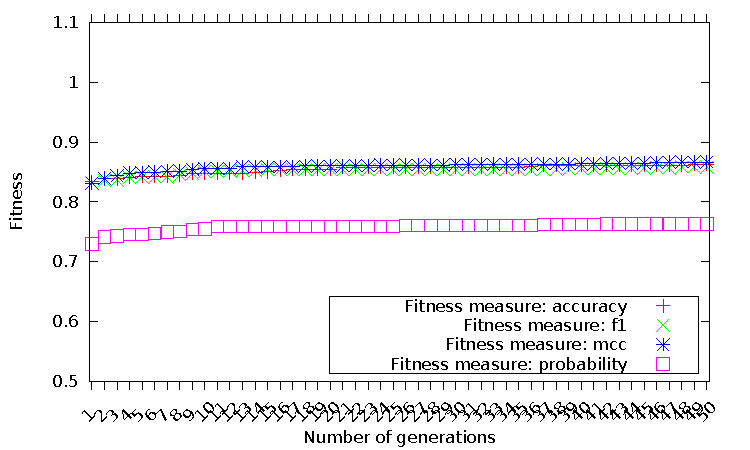
\includegraphics[scale=0.90]{figures/results/fitness/fitness-heart}
		\caption{Najlepsza wartość funkcji przystosowania dla kolejnych pokoleń dla zbioru \emph{heart}.\label{fig:fit-heart}}
	\end{figure}
	
	\begin{figure}
		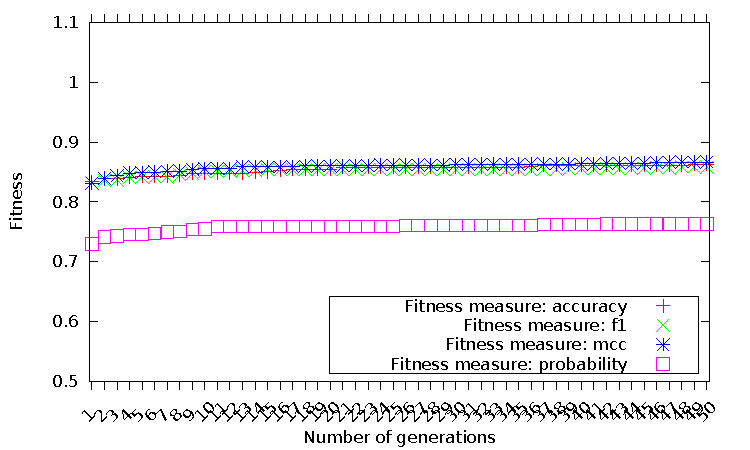
\includegraphics[scale=0.90]{figures/results/fitness/fitness-breast}
		\caption{Najlepsza wartość funkcji przystosowania dla kolejnych pokoleń dla zbioru \emph{breast}.\label{fig:fit-breast}}
	\end{figure}	
	
        \begin{figure}
                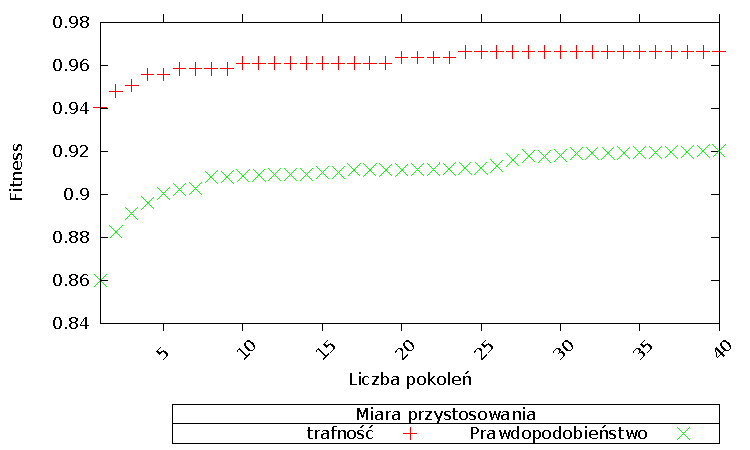
\includegraphics[scale=0.90]{figures/results/fitness/fitness-ionosphere}
                \caption{Najlepsza wartość funkcji przystosowania dla kolejnych pokoleń dla zbioru \emph{ionosphere}.\label{fig:fit-ionosphere}}
        \end{figure}    
               
        \begin{figure}
                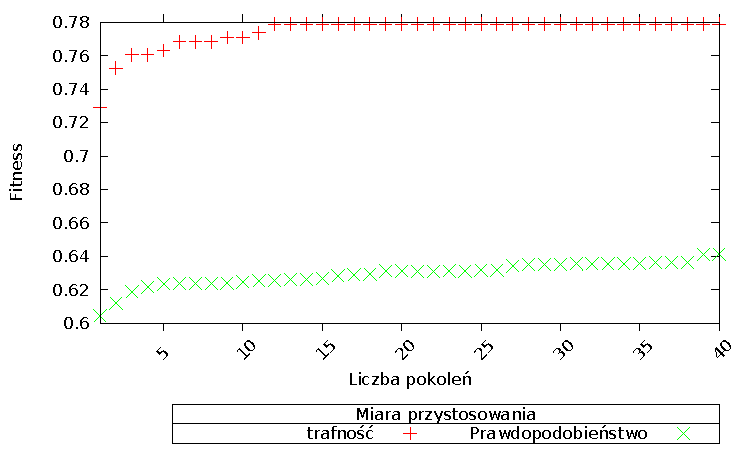
\includegraphics[scale=0.90]{figures/results/fitness/fitness-liver-disorders}
                \caption{Najlepsza wartość funkcji przystosowania dla kolejnych pokoleń dla zbioru \emph{breast}.\label{fig:fit-liver-disorders}}
        \end{figure}    

        \begin{figure}
                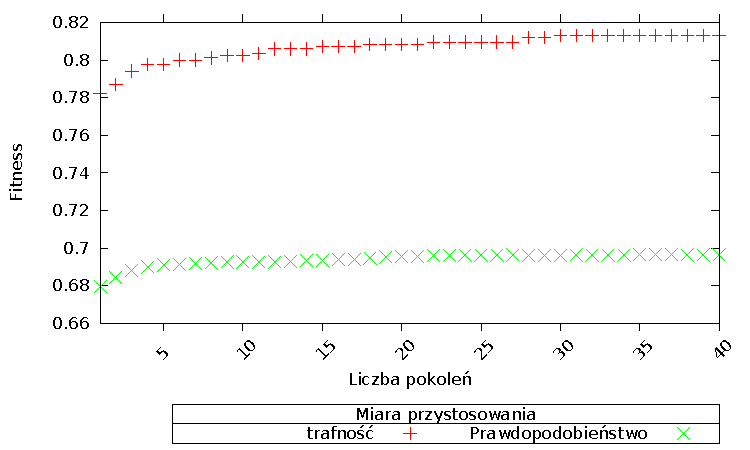
\includegraphics[scale=0.90]{figures/results/fitness/fitness-pima-diabetes}
                \caption{Najlepsza wartość funkcji przystosowania dla kolejnych pokoleń dla zbioru \emph{pima-diabetes}.\label{fig:fit-pima-diabetes}}
        \end{figure}    

	
\FloatBarrier
\section{Wyniki klasyfikacji zbioru testującego}
	Wyniki klasyfikacji zostały ocenione za pomocą miar opisanych w części \ref{sec:measures}. Dla każdej z tych miar przedstawiono jej wartości dla przebiegów algorytmu, w których jako funkcja fitness była wybrana właśnie ta miara. Dodatkowo porównano otrzymane wartości z wynikami uzyskanymi w wyniku klasyfikacji za pomocą trzech standardowych funkcji jądrowych (\emph{Wielomianowej}, \emph{Sigmoidalnej} i \emph{RBF}).
	
	Trafność klasyfikacji osiąganą przez algorytmy pokazano w tabelach \ref{tab:results} i \ref{tab:results2}. Przedstawiono w niej dodatkowo wyniki algorytmów opisanych w części \ref{sec:evokernel}, pochodzące z prac, w których te algorytmy zostały zaprezentowane.
\nprounddigits{3}	
	
%\begin{table}
%	\caption{	\label{tab:results} Zestawienie wyników klasyfikacji. Tabela przedstawia trafność klasyfikacji osiąganą przez poszczególne algorytmy dla przetestowanych zbiorów danych. Wyniki algorytmów K-Tree, Kernel-GP i EKM pochodzą z prac omówionych w rozdziale \ref{sec:evokernel}.}
%%	\begin{tabular}{||r||r|r|r||r|r|r||r||}
%	\begin{tabular}{||l||n{1}{4}|n{1}{4}|n{1}{4}||n{1}{4}|n{1}{4}|n{1}{4}||n{1}{4}||}
%	\hline 
%	& \multicolumn{7}{c||}{Algorytm} \\ 
%	\hline 
%	Zbiór danych & {SMV Poly} & {SVM RBF} & {SVM Sigmoid} & {K-Tree} & {Kernel-GP} & {EKM} & {\textbf{New Kernel-GP}} \\ 
%	\hline \hline
%	{Breast} & 0.97007298 & 0.96569344 & 0.96131387 & • & 0.9546 & 0.97 & 0.95693432 \\ \hline
%	{Heart} & 0.82666667 & 0.82222223 & 0.82888888 & 0.8222 & 0.7759 & • & 0.82888889 \\ \hline
%	{Ionosphere} & 0.87521368 & 0.93504274 & 0.87008548 & 0.943 & 0.9404 & 0.905 & 0.84615386 \\ \hline
%	{Liver} & 0.61217391 & 0.59652172 & 0.60347826 & 0.7227 & • & 0.691 & 0.68173914 \\ \hline
%	{Pima} & 0.74609375 & 0.75546875 & 0.73203125 & 0.7747 & • & 0.748 & 0.76015625 \\ \hline
%	\end{tabular} 	
%\end{table}


\begin{table}
	\caption{	\label{tab:results} Zestawienie wyników klasyfikacji. Tabela przedstawia trafność klasyfikacji osiąganą przez LibSVM dla różnych funkcji jądrowych przy domyślnych ustawieniach oraz wyniki uzyskane za pomocą przeszukiwania Grid Search dostępnego wraz z biblioteką LibSVM.}
	\begin{tabular}{|l||n{1}{4}|n{1}{4}|n{1}{4}||n{1}{4}||}
	\hline
	 & \multicolumn{4}{c||}{Algorytm} \\ 	
	\hline \hline
	Zbiór & {LibSVM Polly} & {LibSVM RBF} & {LibSVM Sigmoid} & {Grid LibSVM} \\ \hline
	Breast & 0.970 & 0.966 & 0.961 & 0.972 \\ \hline
	Heart & 0.827 & 0.822 & 0.829 & 0.844 \\ \hline
	Ionosphere & 0.875 & 0.935 & 0.870 & 0.952 \\ \hline
	Liver & 0.612 & 0.597 & 0.603 & 0.739 \\ \hline
	Pima & 0.746 & 0.755 & 0.732 & 0.777 \\ \hline
	\end{tabular} 	
\end{table}

\begin{table}
	\caption{	\label{tab:results2} Zestawienie wyników klasyfikacji. Tabela przedstawia trafność klasyfikacji osiąganą przez poszczególne algorytmy dla przetestowanych zbiorów danych. Wyniki algorytmów K-Tree, Kernel-GP i EKM pochodzą z prac omówionych w rozdziale \ref{sec:evokernel}.}
	\begin{tabular}{||r||n{1}{4}||n{1}{4}|n{1}{4}|n{1}{4}||n{1}{4}||}
	\hline 
	 & \multicolumn{5}{c||}{Algorytm} \\ 
	\hline 
	Zbiór danych & {Grid LibSVM} & {K-Tree} & {Kernel-GP} & {EKM} & \textbf{New Kernel-GP} \\ 
	\hline \hline
	Breast & 0.972 & • & 0.955 & 0.970 & 0.97222932 \\ \hline
	Heart & 0.844 & 0.822 & 0.776 &  • &  0.84074075 \\ \hline
	Ionosphere & 0.952 & 0.943 & 0.940 & 0.905 & 0.93162 \\ \hline
	Liver & 0.739 & 0.723 & • & 0.691 & 0.70495799 \\ \hline
	Pima & 0.777 & 0.775 & • & 0.748 & 0.77266 \\ \hline
	\end{tabular} 	
\end{table}


%\begin{table}[htbp]
%\caption{Średnia wartość prawdopodobieństwa przypisana właściwej klasie}
%\begin{center}
%	\begin{tabular}{|l||n{1}{4}|n{1}{4}|n{1}{4}|n{1}{4}|}
%		\hline 
%		& \multicolumn{4}{c|}{Algorytm} \\ 
%		\hline
%		Zbiór danych & {SMV Poly} & {SVM RBF} & {SVM Sigmoid} & {New KernelGP} \\ \hline \hline
%		Breast & 0.952839 & 0.951593 & 0.946545 & •  \\ \hline
%		Heart & 0.737089 & 0.752142 & 0.759086 & •  \\ \hline
%		Ionosphere & 0.793675 & 0.901037 & 0.750996 & 0.902296 \\ \hline
%		Liver & 0.537505 & 0.537623 & 0.530987 & 0.584991 \\ \hline
%		Pima & 0.645106 & 0.68108 & 0.657695 & 0.676421 \\ \hline
%	\end{tabular}
%\end{center}
%\label{tab:results-prob}
%\end{table}



	
	Jak widać na rysunkach \ref{fig:acc-breast}-\ref{fig:probability-heart} sprawność algorytmu zależy zarówno od zbioru danych jak i od wybranej miary jakości.
	
	\begin{figure}
		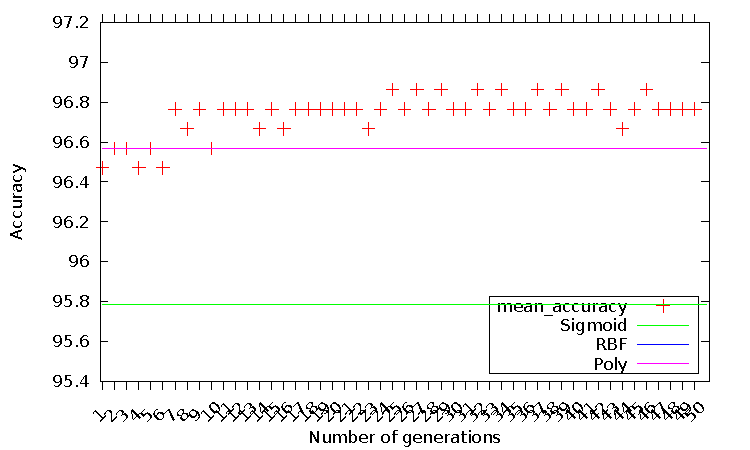
\includegraphics[scale=0.90]{figures/results/accuracy/accuracy-breast}
		\caption{Trafność (\english{accuracy}) klasyfikacji dla zbioru \emph{breast} w funkcji czasu wykonania (ilości pokoleń).\label{fig:acc-breast}}
	\end{figure}
	
	\begin{figure}
		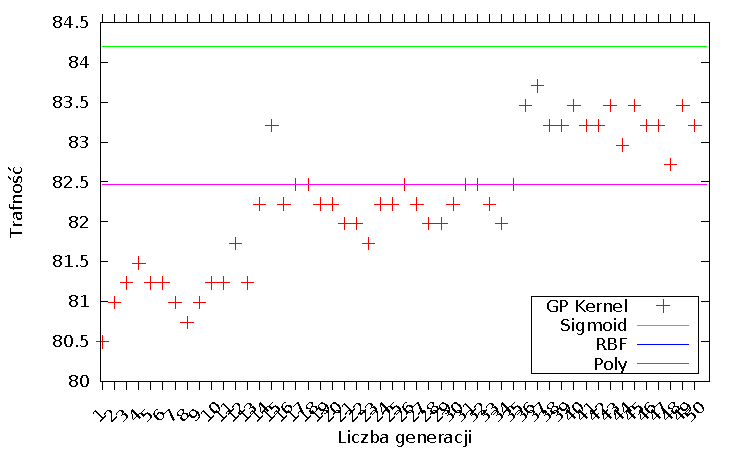
\includegraphics[scale=0.90]{figures/results/accuracy/accuracy-heart}
		\caption{Trafność (\english{accuracy}) klasyfikacji dla zbioru \emph{heart} w funkcji czasu wykonania (ilości pokoleń).\label{fig:acc-heart}}
	\end{figure}
	
	\begin{figure}
		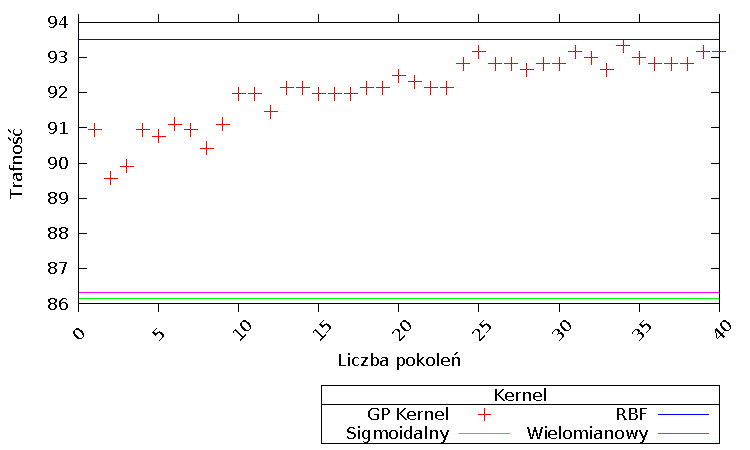
\includegraphics[scale=0.90]{figures/results/accuracy/accuracy-ionosphere}
		\caption{Trafność (\english{accuracy}) klasyfikacji dla zbioru \emph{ionosphere} w funkcji czasu wykonania (ilości pokoleń).\label{fig:acc-ionosphere}}
	\end{figure}
	
	\begin{figure}
		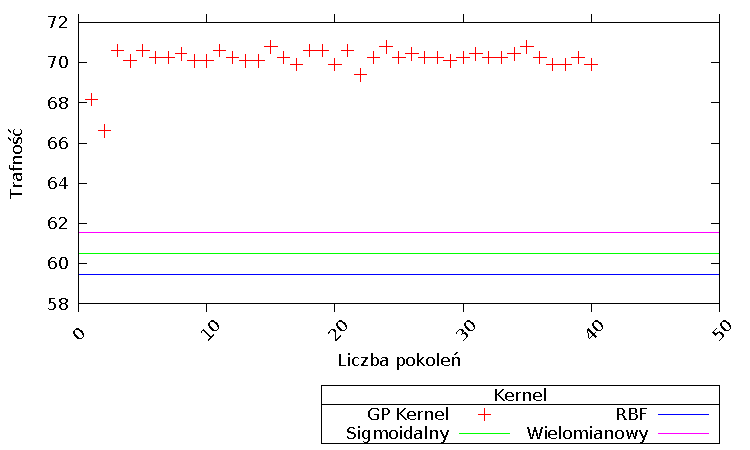
\includegraphics[scale=0.90]{figures/results/accuracy/accuracy-liver-disorders}
		\caption{Trafność (\english{accuracy}) klasyfikacji dla zbioru \emph{liver} w funkcji czasu wykonania (ilości pokoleń).\label{fig:acc-liver}}
	\end{figure}
		
	\begin{figure}
		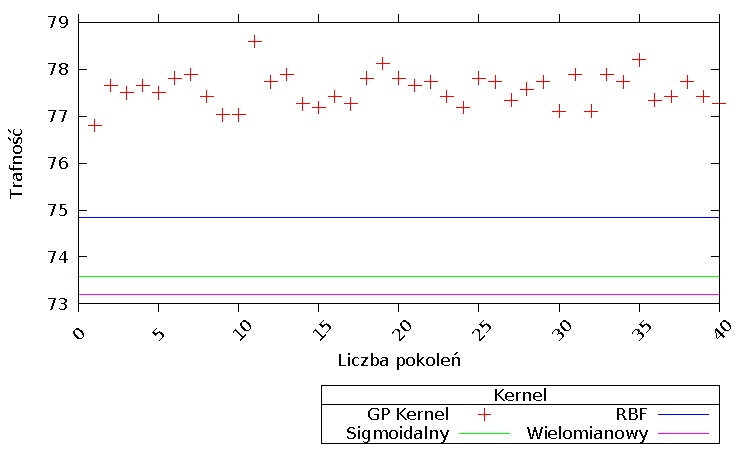
\includegraphics[scale=0.90]{figures/results/accuracy/accuracy-pima-diabetes}
		\caption{Trafność (\english{accuracy}) klasyfikacji dla zbioru \emph{pima} w funkcji czasu wykonania (ilości pokoleń).\label{fig:acc-pima}}
	\end{figure} 
	
	\begin{figure}
		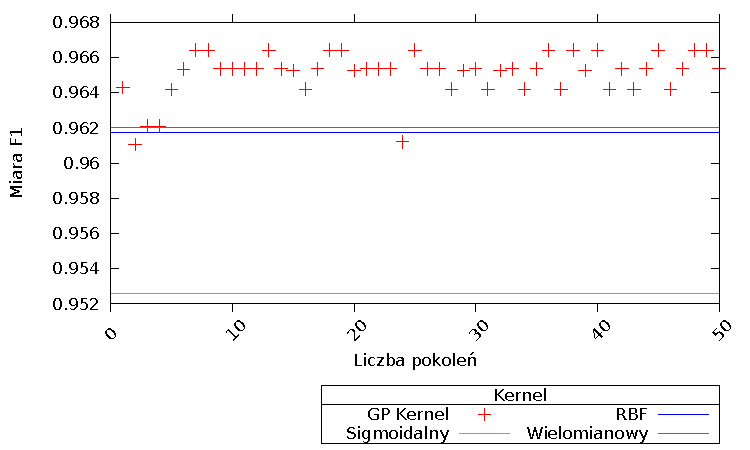
\includegraphics[scale=0.90]{figures/results/f1/f1-breast}
		\caption{Wartość miary F1 dla wyników klasyfikacji zbioru \emph{breast} w funkcji czasu wykonania (ilości pokoleń).\label{fig:f1-breast}}
	\end{figure}
	
	\begin{figure}
		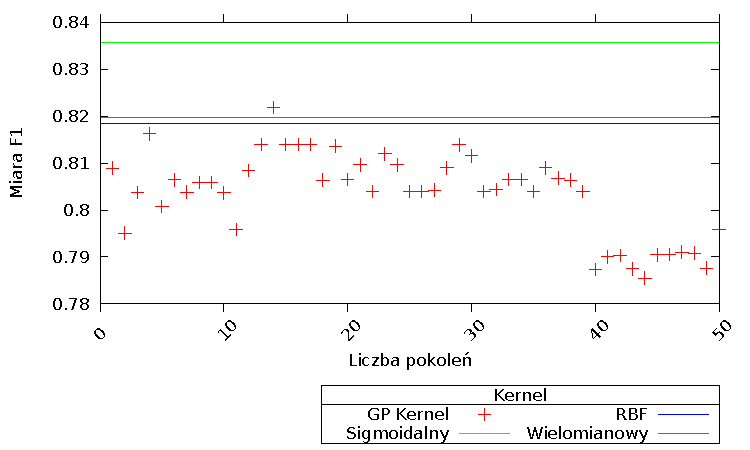
\includegraphics[scale=0.90]{figures/results/f1/f1-heart}
		\caption{Wartość miary F1 dla wyników klasyfikacji zbioru \emph{heart} w funkcji czasu wykonania (ilości pokoleń).\label{fig:f1-heart}}
	\end{figure}
	
	\begin{figure}
		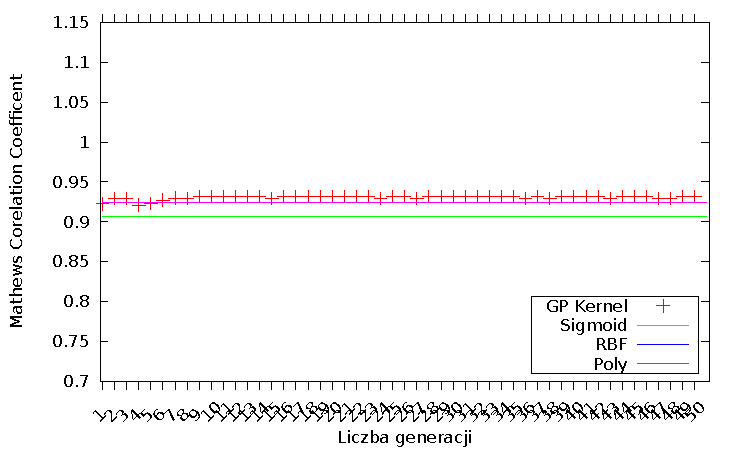
\includegraphics[scale=0.90]{figures/results/mcc/mcc-breast}
		\caption{Wartość miary \emph{Mathews Correlation Coefficent} (\akronim{mcc}) dla wyników klasyfikacji zbioru \emph{breast} w funkcji czasu wykonania (ilości pokoleń).\label{fig:mcc-breast}}
	\end{figure}
	
	\begin{figure}
		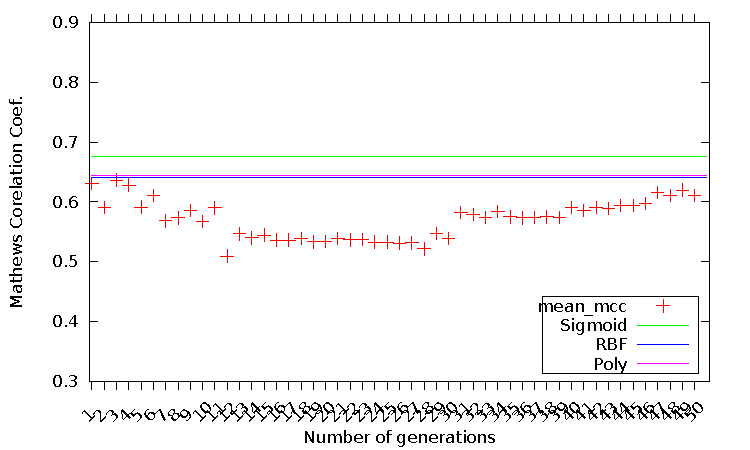
\includegraphics[scale=0.90]{figures/results/mcc/mcc-heart}
		\caption{Wartość miary \emph{Mathews Correlation Coefficent} dla wyników klasyfikacji zbioru \emph{heart} w funkcji czasu wykonania (ilości pokoleń).\label{fig:mcc-heart}}
	\end{figure}
	
	\begin{figure}
		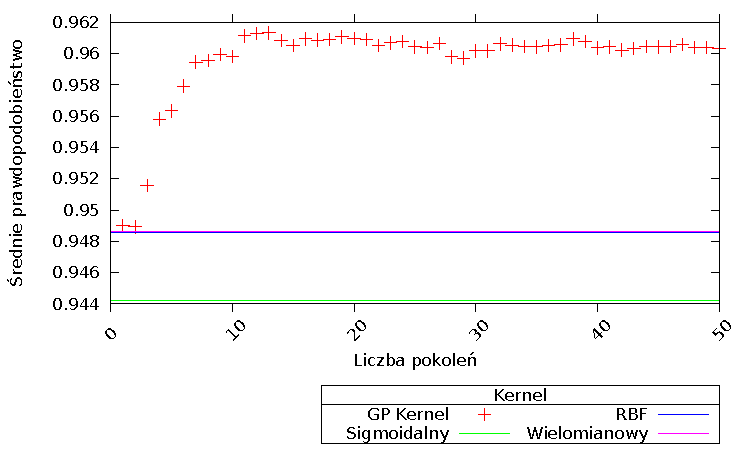
\includegraphics[scale=0.90]{figures/results/probability/probability-breast}
		\caption{Średnia wartość prawdopodobieństwa przypisywanego przez SVM właściwej dla klasyfikowanego przykłau klasie w funkcji czasu wykonania (ilości pokoleń). Zbiór \emph{breast}\label{fig:probability-breast}}
	\end{figure}
	
	\begin{figure}
		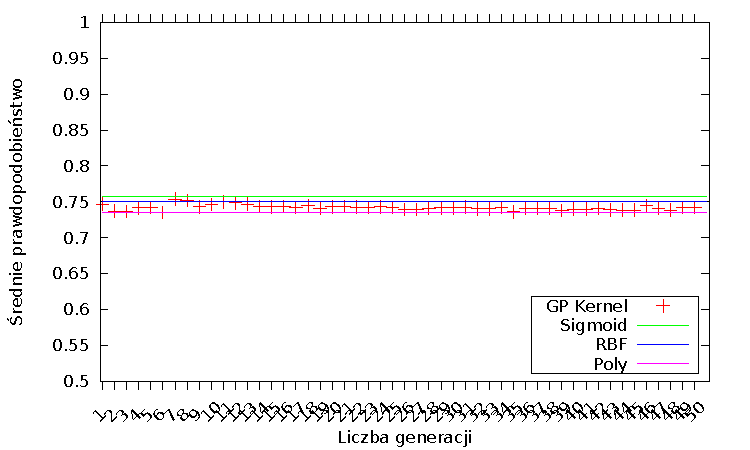
\includegraphics[scale=0.90]{figures/results/probability/probability-heart}
		\caption{Średnia wartość prawdopodobieństwa przypisywanego przez SVM właściwej dla klasyfikowanego przykłau klasie w funkcji czasu wykonania (ilości pokoleń). Zbiór \emph{heart}.\label{fig:probability-heart}}
	\end{figure}
	
                \begin{figure}
                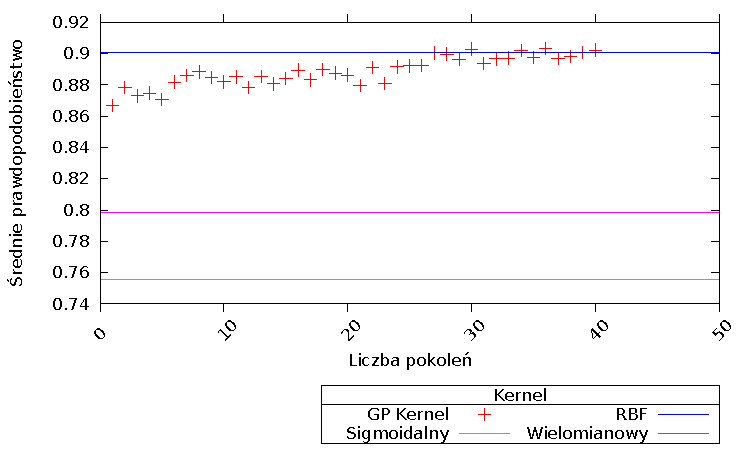
\includegraphics[scale=0.90]{figures/results/probability/probability-ionosphere}
                \caption{Średnia wartość prawdopodobieństwa przypisywanego przez SVM właściwej dla klasyfikowanego przykłau klasie w funkcji czasu wykonania (ilości pokoleń). Zbiór \emph{ionosphere}.\label{fig:probability-ionosphere}}
        \end{figure}


        \begin{figure}
                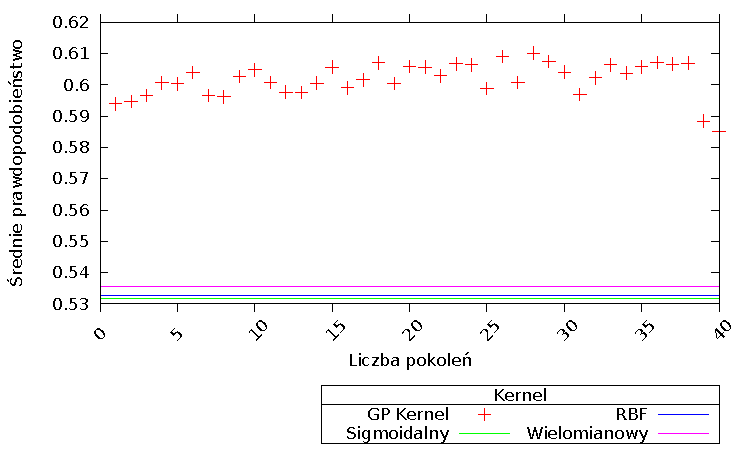
\includegraphics[scale=0.90]{figures/results/probability/probability-liver-disorders}
                \caption{Średnia wartość prawdopodobieństwa przypisywanego przez SVM właściwej dla klasyfikowanego przykłau klasie w funkcji czasu wykonania (ilości pokoleń). Zbiór \emph{liver-disorders}.\label{fig:probability-liver-disorders}}
        \end{figure}


        \begin{figure}
                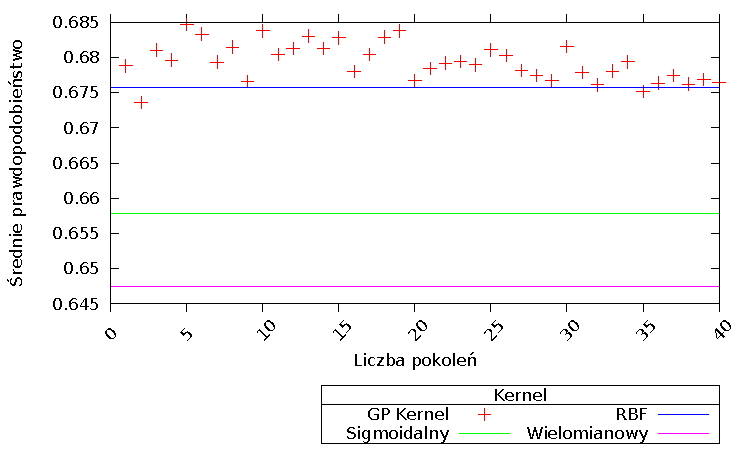
\includegraphics[scale=0.90]{figures/results/probability/probability-pima-diabetes}
                \caption{Średnia wartość prawdopodobieństwa przypisywanego przez SVM właściwej dla klasyfikowanego przykłau klasie w funkcji czasu wykonania (ilości pokoleń). Zbiór \emph{pima-diabetes}.\label{fig:probability-pima-diabetes}}
        \end{figure}



%	\subsection{Porównanie z tradycyjnym algorytmem SVM}
%	Na wykresach \ref{fig:acc-iris-svm}-\ref{fig:acc-letter-svm} przedstawiono porównanie trafności klasyfikacji zbioru walidującego przez algorytm SVM z użyciem czterech podstawowych funkcji jądrowych (liniowej, wielomianowej, RBF i sigmoidalnej) i przez stworzony algorytm Kernel-GP.
%	W przypadku dwóch zbiorów: \emph{vowel} i \emph{letter} udało się uzyskać polepszenie trafności klasyfikacji względem standardowych funkcji jądrowych. Są to zbiory, dla których standardoy SVM osiąga słabe wyniki - ok. $ 70\% - 80\% $. 
%
%	W przypadku dwóch pozostałych zbiorów niezależnie od użytej funkcji jądrowej osiągana trafność klasyfikacji jest bardzo wysoka - ok. $ 95\% $ - sugeruje to, że zbiory te są dość łatwo separowalne z wyjątkiem $ 5\% $ przypadków.
	
%	\begin{figure}
%		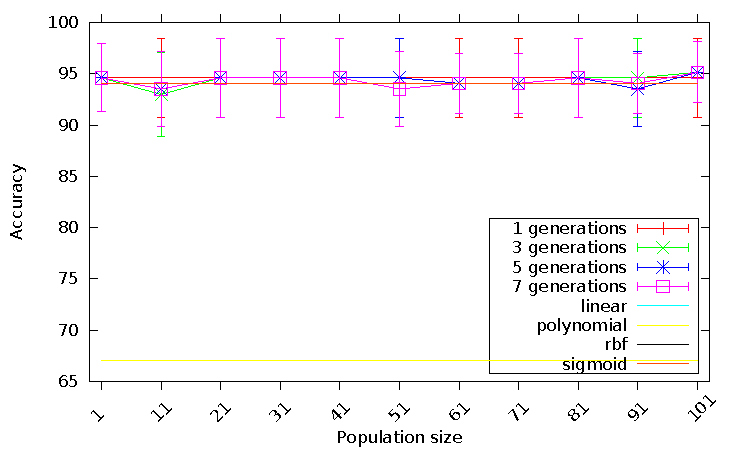
\includegraphics[scale=0.90]{figures/results/accuracy/accuracy-iris-svm}
%		\caption{Porównanie trafności klasyfikacji dla zbioru \emph{iris} przez algorytm SVM z różnymi funkcjami jądrowymi i algorytm Kernel-GP\label{fig:acc-iris-svm}}
%	\end{figure}
%	
%	\begin{figure}
%		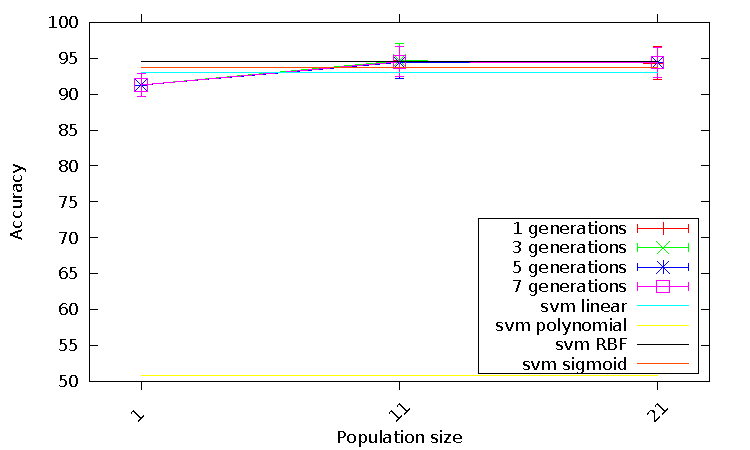
\includegraphics[scale=0.90]{figures/results/accuracy/accuracy-dna-svm}
%		\caption{Porównanie trafności klasyfikacji dla zbioru \emph{dna} przez algorytm SVM z różnymi funkcjami jądrowymi i algorytm Kernel-GP.\label{fig:acc-dna-svm}}
%	\end{figure}	
%	
%	\begin{figure}
%		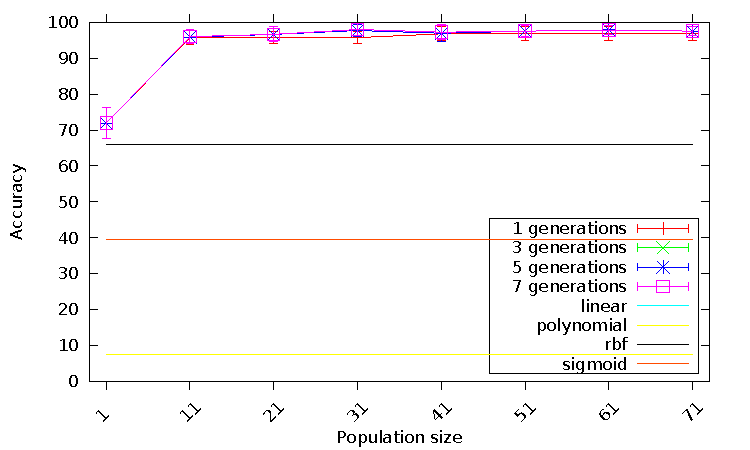
\includegraphics[scale=0.90]{figures/results/accuracy/accuracy-vowel-svm}
%		\caption{Porównanie trafności klasyfikacji dla zbioru \emph{vowel} przez algorytm SVM z różnymi funkcjami jądrowymi i algorytm Kernel-GP\label{fig:acc-vowel-svm}}
%	\end{figure}
%	
%	\begin{figure}
%		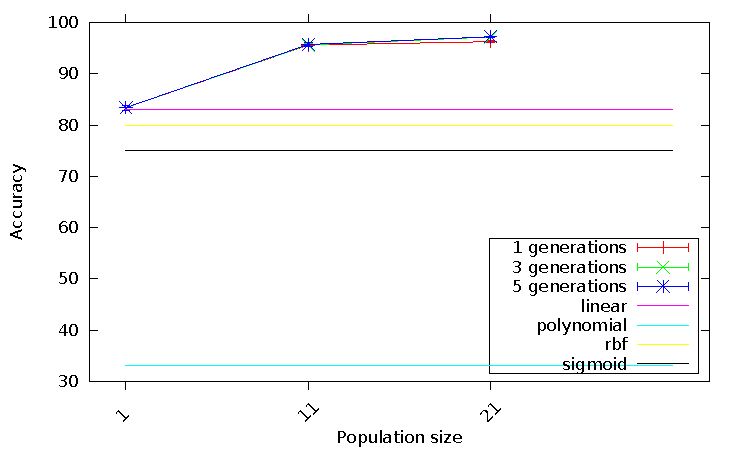
\includegraphics[scale=0.90]{figures/results/accuracy/accuracy-letter-svm}
%		\caption{Porównanie trafności klasyfikacji dla zbioru \emph{letter} przez algorytm SVM z różnymi funkcjami jądrowymi i algorytm Kernel-GP\label{fig:acc-letter-svm}}
%	\end{figure}		
%
%\FloatBarrier
%	\subsection{Monotoniczność funkcji trafności}	
%	Miejscami funkcja trafności nie jest monotoniczna, a ściślej niemalejąca, względem liczby pokoleń oraz wielkości populacji (co widać np. na wykresach \ref{fig:acc-iris-detailed} i \ref{fig:acc-vowel-detailed}). Wydawałoby się, że tak być nie powinno (algorytm genetyczny zwraca najlepszego osobnika z całego swojego przebiegu, więc wszystkie osobniki, które pojawiły się w pierwszych 5 pokoleniach pojawią się w pierwszych 7 pokoleniach, więc trafność dla po 7 pokoleniach powinna być co najmniej tak dobra jak po 5). Jednak może się tak zdarzyć ze względu na to, że trafność pokazana na wykresach to trafność klasyfikacji zbioru walidującego, natomiast trafność użyta przez algorytm genetyczny jako miara dostosowania (\english{fitness}) to trafność klasyfikacji zbioru testującego. Widać to na wykresie \ref{fig:fit-iris-detailed}, który przedstawia wartość przystosowania dla tych samych danych, dla których na wykresie \ref{fig:acc-iris-detailed} jest pokazana trafność klasyfikacji na zbiorze walidującym - tutaj funkcja wykazuje mniej braku monotoniczności. 
%
%%	\begin{figure}
%%		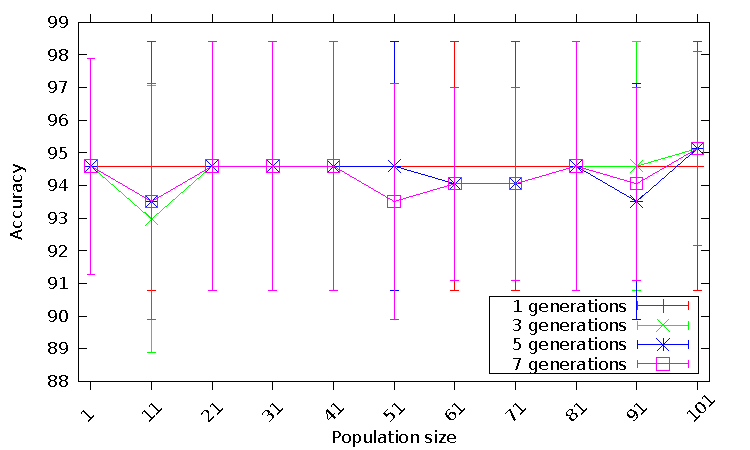
\includegraphics[scale=0.90]{figures/results/accuracy/accuracy-iris}
%%		\caption{Trafność klasyfikacji dla zbioru \emph{iris} w funkcji rozmiaru populacji dla róznych ilości pokoleń.\label{fig:acc-iris}}
%%	\end{figure}
%%	
%	\begin{figure}
%		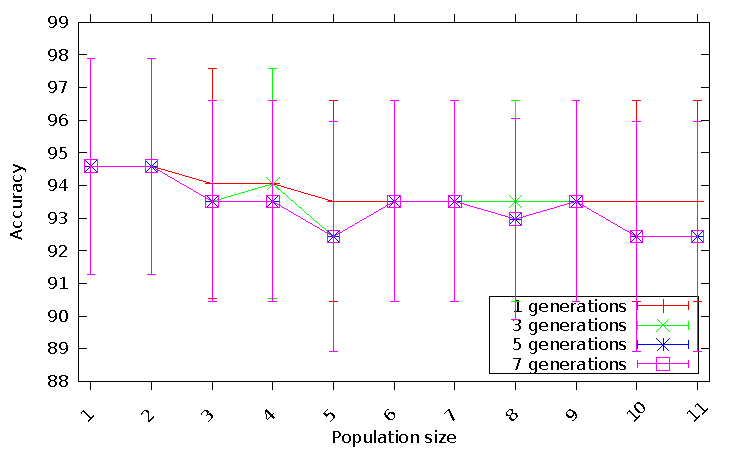
\includegraphics[scale=0.90]{figures/results/accuracy/accuracy-iris-detailed}
%		\caption{Trafność klasyfikacji dla zbioru \emph{iris} w funkcji rozmiaru populacji dla róznych ilości pokoleń, dla małych populacji.	\label{fig:acc-iris-detailed}}
%	\end{figure}	
%	
%	
%	\begin{figure}
%		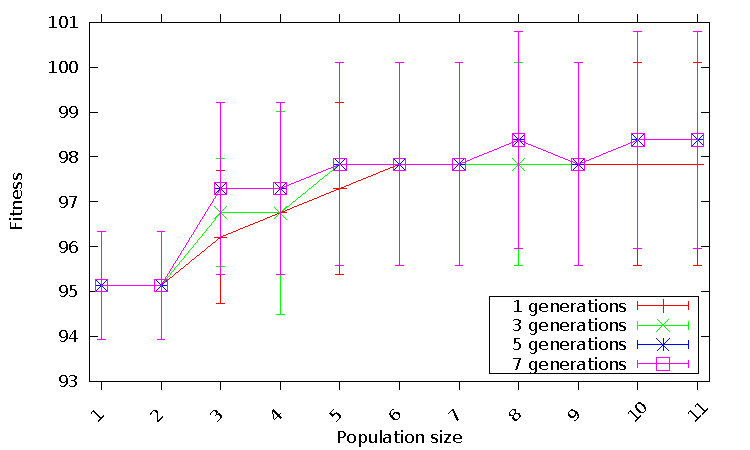
\includegraphics[scale=0.90]{figures/results/fitness/fitness-iris-detailed}
%		\caption{Najlepsza wartość funkcji przystosowania (\english{fitness})  \emph{iris} w funkcji rozmiaru populacji dla róznych ilości pokoleń, dla małych populacji.	\label{fig:fit-iris-detailed}}
%	\end{figure}	
%	
%%	
%%	\begin{figure}
%%		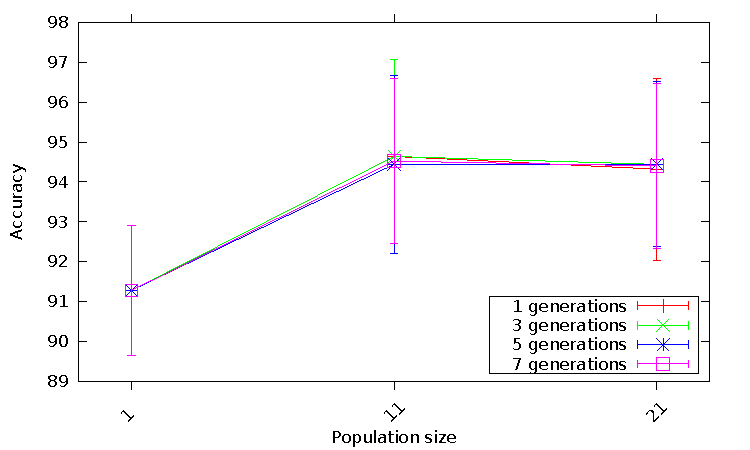
\includegraphics[scale=0.90]{figures/results/accuracy/accuracy-dna}
%%		\caption{Trafność klasyfikacji dla zbioru \emph{DNA} w funkcji rozmiaru populacji dla róznych ilości pokoleń.\label{fig:acc-dna}}
%%	\end{figure}
%%	
%%	\begin{figure}
%%		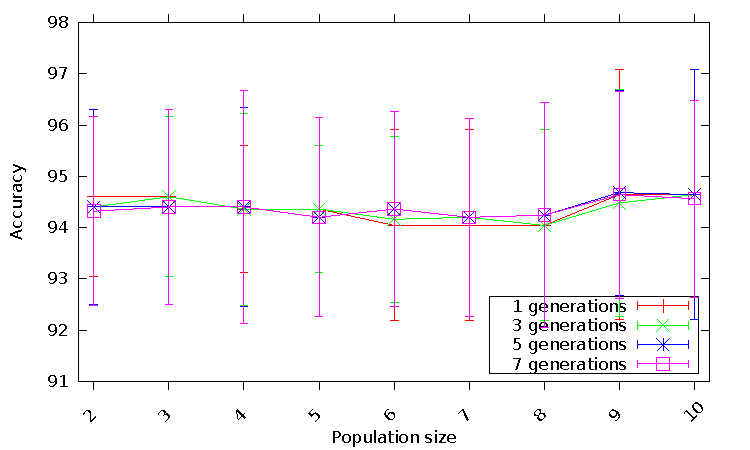
\includegraphics[scale=0.90]{figures/results/accuracy/accuracy-dna-detailed}
%%		\caption{Trafność klasyfikacji dla zbioru \emph{DNA} w funkcji rozmiaru populacji dla róznych ilości pokoleń, dla małych populacji.\label{fig:acc-dna-detailed}}
%%	\end{figure}	
%%	
%%
%%	\begin{figure}
%%		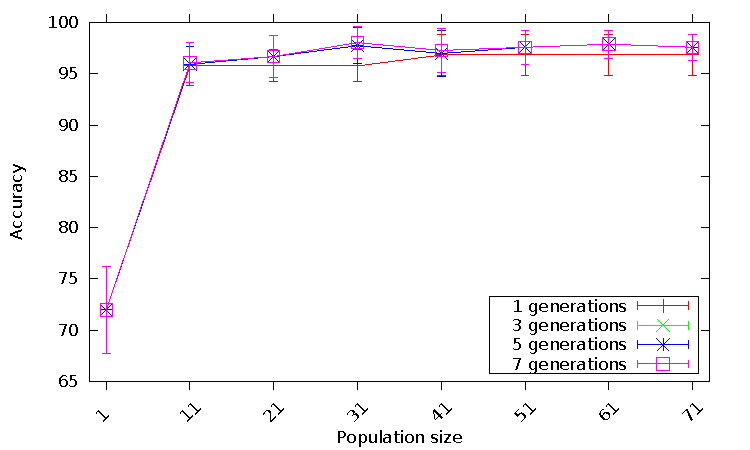
\includegraphics[scale=0.90]{figures/results/accuracy/accuracy-vowel}
%%		\caption{Trafność klasyfikacji dla zbioru \emph{vowel} w funkcji rozmiaru populacji dla róznych ilości pokoleń.\label{fig:acc-vowel}}
%%	\end{figure}
%		%	
%%	
%%		\begin{figure}
%%		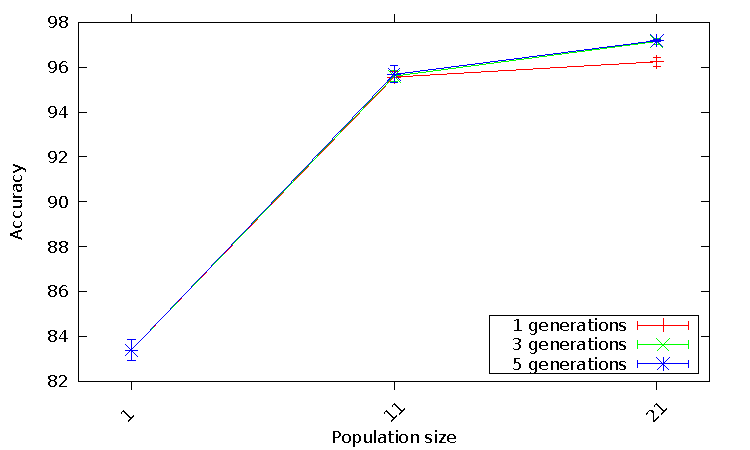
\includegraphics[scale=0.90]{figures/results/accuracy/accuracy-letter}
%%		\caption{Trafność klasyfikacji dla zbioru \emph{letter} w funkcji rozmiaru populacji dla róznych ilości pokoleń.\label{fig:acc-letter}}
%%	\end{figure}
%%	
%%		
%%	\begin{figure}
%%		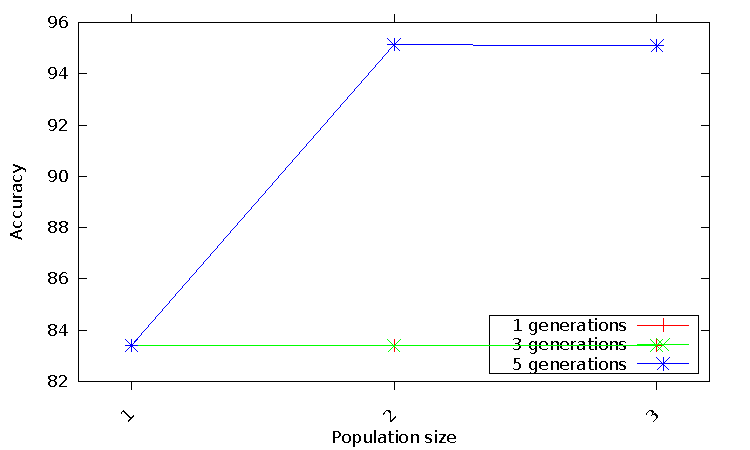
\includegraphics[scale=0.90]{figures/results/accuracy/accuracy-letter-detailed}
%%		\caption{Trafność klasyfikacji dla zbioru \emph{letter} w funkcji rozmiaru populacji dla róznych ilości pokoleń, dla małych populacji.\label{fig:acc-letter-detailed}}
%%	\end{figure}
%%	
%
%	\FloatBarrier
%	Zatem przynajmniej część braku monotoniczności funkcji trafności na zbiorze walidującym wynika z przeuczenia algorytmu - znaleziona przez algorytm genetyczny funkcja jądrowa lepiej sprawdza się przy klasyfikacji zbioru testującego niż walidującego. Nie jest to jednak jedyna przyczyna braku monotoniczności - widać to na wykresie \ref{fig:fit-vowel-detailed} przedstawiającym wartość funkcji przystosowania dla zbioru \emph{vowel} - jej przebieg jest bardzo podobny do przebiegu ukazanej na rys. \ref{fig:acc-vowel-detailed} funkcji trafności klasyfikacji zbioru walidującego na tym samym zbiorze. Co więc jest przyczyną braku monotoniczności? Warto zauważyć, że funkcja jest niemalejąca ze względu na ilość pokoleń oraz że dla jednego pokolenia funkcja jest monotoniczna. Sugeruje to, że "winnym" może być selekcja - w praktyce nie zachodzi ono w przypadku gdy algorytm genetyczny działa przez jedno pokolenie.
%
%	\begin{figure}
%		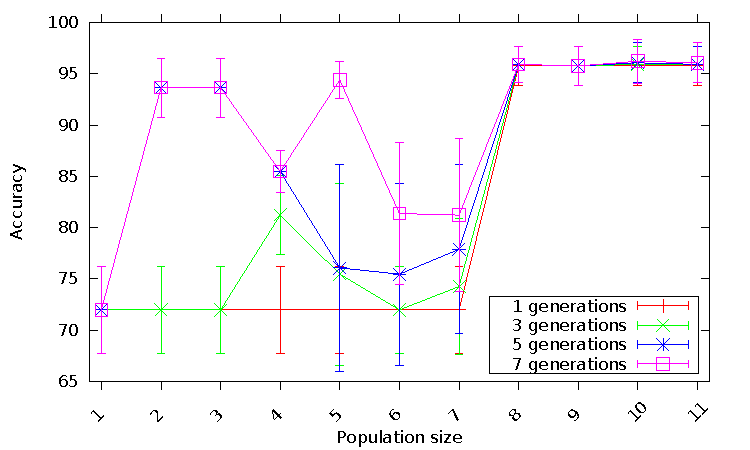
\includegraphics[scale=0.90]{figures/results/accuracy/accuracy-vowel-detailed}
%		\caption{Trafność klasyfikacji dla zbioru \emph{vowel} w funkcji rozmiaru populacji dla róznych ilości pokoleń, dla małych populacji.\label{fig:acc-vowel-detailed}}
%	\end{figure}
%		
%	\begin{figure}
%		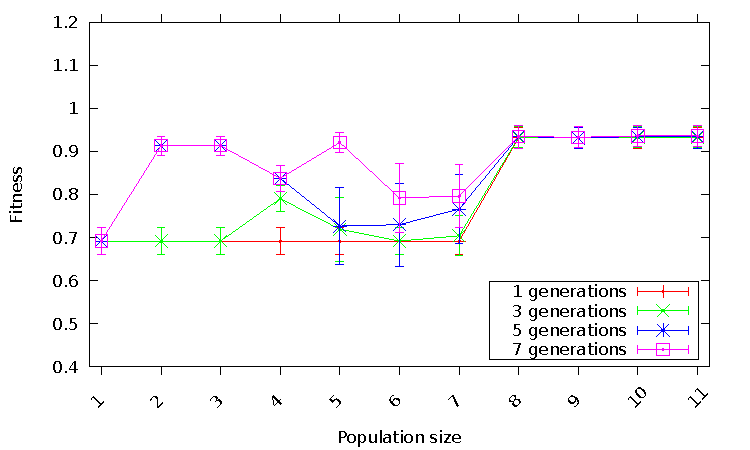
\includegraphics[scale=0.90]{figures/results/fitness/fitness-vowel-detailed}
%		\caption{Trafność klasyfikacji dla zbioru \emph{vowel} w funkcji rozmiaru populacji dla róznych ilości pokoleń, dla małych populacji.\label{fig:fit-vowel-detailed}}
%	\end{figure}
%
%    	
%	\FloatBarrier
%	 Gdy przyjrzeć się dokładnie przebiegowi ewolucji widać, że rzeczywiści tak jest. Dodatkowy osobnik (rys. \ref{fig:func1}), który odróżnia w pokoleniu pierwszym populacje o wielkości 3 i 4 jest przodkiem innego osobnika (rys. \ref{fig:func2}), który w trzecim pokoleniu osiąga fitness większy niż osobnik (rys. \ref{fig:func3}), który w przypadku populacji wielkości 3 był przodkiem osobnika (rys. \ref{fig:func4}), który to okazał się najlepszym podczas przebiegu całego algorytmu. W rezultacie tego "geny" potencjalnego zwycięzcy nie przetrwały w przebiegu algorytmu z populacją liczącą 4 osobników. Jak widać osobnik najlepszy we wszystkich pokoleniach nie musi być wcale potomkiem osobników najlepszych w poszczególnych pokoleniach - czasem połączenie dwóch osobników przeciętnych może dać osobnika bardzo dobrego. 	
%	 
%	     \begin{figure}
%		
\includegraphics[scale=0.50]{figures/functions/func1}
%		\caption{Funkcja z pierwszego pokolenia, która w przebiego z wielkością populacji 4 osiągnęła fitness $0.4242424$. Przodek funkcji z rys.\ref{fig:func2} \label{fig:func1}}
%	\end{figure}
%	
%	\begin{figure}
%		
\includegraphics[scale=0.60]{figures/functions/func2}
%		\caption{Funkcja z trzeciego pokolenia, która w przebiego z wielkością populacji 4 osiągnęła fitness $0.78030306$. Potomek funkcji z rys.\ref{fig:func1}, przodek zwycięskiej funkcji (rys.\ref{fig:func5}) z przebiegu z populacją o wielkości 4.\label{fig:func2}}
%	\end{figure}
%          
%   	\begin{figure}
%		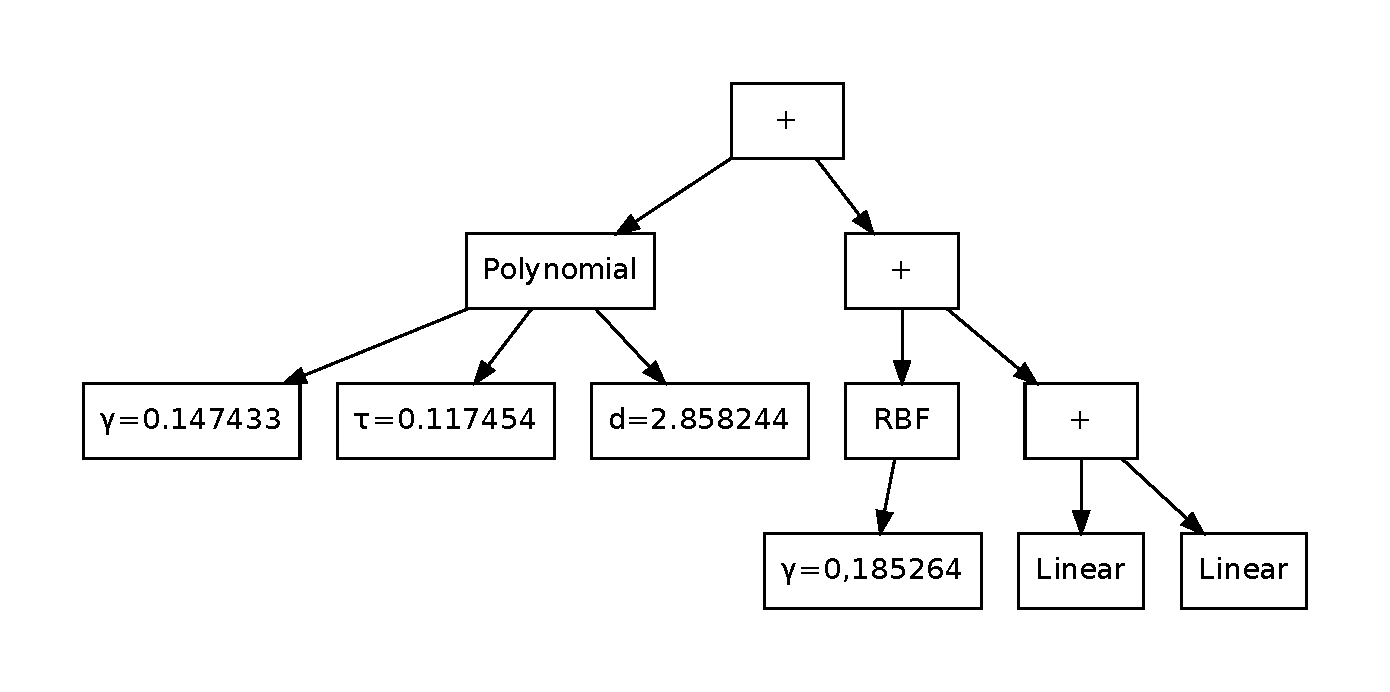
\includegraphics[scale=0.60]{figures/functions/func5}
%		\caption{Funkcja z ostatniego pokolenia w przebiegu z wielkością populacji 4 osiągnęła fitness $0.8333333$. Przodek zwycięskiej funkcji z rys.\ref{fig:func4} \label{fig:func5}}
%	\end{figure}          
%
%
%   	\begin{figure}
%		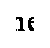
\includegraphics[scale=0.60]{figures/functions/func3}
%		\caption{Funkcja z trzeciego pokolenia, która w przebiegu z wielkością populacji 3 i 4 osiągnęła fitness $0.6515151$. Przodek zwycięskiej funkcji z rys.\ref{fig:func4}\label{fig:func3}}
%	\end{figure}                 
%
%    	\begin{figure}
%		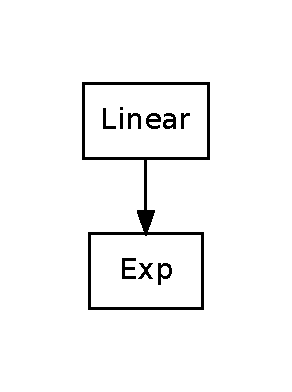
\includegraphics[scale=0.60]{figures/functions/func4}
%		\caption{Zwycięska funkcja w przebiegu z populacją wielkości 3, potomek funkcji z rys.\ref{fig:func3}. Osiągnęła fitness $0.9015151$. \label{fig:func4}}
%	\end{figure} 
%

		


\section{Czas wykonania}

Główną wadą proponowanego podejścia są spore czasy wykonania algorytmu. Algorytm programowania genetycznego uruchamia klasyfikator SVM, najpierw w trybie uczenia, potem klasyfikacji, za każdym razem kiedy dokonuje ewaluacji (oceny) osobnika, czyli $ G \times P $ razy, gdzie $ P $ to wielkość populacji a $ G $ liczba pokoleń przez które działa algorytm. Dla parametrów używanych najczęściej podczas przeprowadzonych eksperymentów, czyli $ P = 100 $ i $ G = 50 $ daje to $ 5000 $ wywołań \emph{LibSVM}. Do tego należy jeszcze doliczyć narzut związany z operacjami selekcji, mutacji i krzyżowania dokonywanymi przez \emph{ECJ}. Dodatkowo można się spodziewać, że obliczenie wartości zwracanej przez funkcję jądrową będzie, dla tej samej funkcji, bardziej czasochłonne kiedy jest ona obliczana przez \emph{ECJ} jako wartość drzewa , niż w przypadku, kiedy jest ona liczona jako wartość wyrażenia Javy zapisanego w \emph{LibSVM} - ze względu na narzut związany z przechodzeniem przez  gałęzie drzewa. Co więcej funkcje jądrowe generowane przez GP z założenia są kombinacją kilku standardowych funkcji jądrowych, a więc wymagają większej liczby obliczeń.

W celu przeanalizowania źródła czasochłonności obliczeń Kernel-GP podczas przeprowadzania eksperymentów zapisywano czas ich wykonania. Wyniki przedstawiają tabele \ref{tab:results-time-LSVM} oraz \ref{tab:results-time-GP} a także wykresy \ref{fig:time-all-breast} i \ref{fig:time-some-breast}.

Patrząc na wykresy \ref{fig:time-all-breast} i \ref{fig:time-some-breast} widać, że narzut związany z mechanizmami algorytmu GP nie jest znaczący. Problem stanowi spora zmienność czasów wykonania algorytmu Kernel-GP - odchylenie standardowe czasu wykonania czasami jest większe niż średnia. Jest to przypuszczalnie spowodowane użyciem funkcji jądrowych, które nie są dodatnio określone (na przykład funkcja sigmoidalna) i dla których rozwiązywany przez SVM problem optymalizacji może nie być wypukły. Czas wykonania nie rośnie liniowo wraz z liczbą dokonywanych ocen generowanych funkcji - dla 10 pokoleń wielkości 10 osobników, a więc 100 ewaluacji, czas wykonania jest co najwyżej 10 razy większy niż przy jednym osobniku i jednym pokoleniu, czyli 1 ewaluacji. Jest to spowodowane pewnym stałym kosztem obliczeniowym  związanym z inicjalizacją procesu ewolucyjnego, która wykonuje się tylko raz oraz z tym, że osobniki identyczne do już ocenianych nie są oceniane po raz drugi. Im proces ewolucyjny trwa dłużej, tym bardziej homogeniczna staje się populacja a co za tym idzie więcej występuje w niej identycznych osobników.

\begin{table}[htbp]
\caption{Czasy uczenia na zbiorze uczącym i klasyfikacji zbioru testującego przez klasyfikator LibSVM.}
\begin{tabular}{|l|c|c|c|c|}
\hline
 & \multicolumn{ 4}{c|}{LibSVM kernels} \\ \hline
dataset & LibSVM linear & LibSVM polynomial & LibSVM rbf & LibSVM Sigmoid \\ \hline
breast & $ 0.55\pm 0.05 $ & $ 0.59\pm 0.04 $ & $ 0.51\pm 0.04 $ & $ 0.52\pm 0.05 $ \\ \hline
heart & $ 0.53\pm 0.03 $ & $ 0.55\pm 0.05 $ & $ 0.48\pm 0.03 $ & $ 0.49\pm 0.05 $ \\ \hline
ionosphere & $ 0.78\pm 0.02 $ & $ 0.82\pm 0.03 $ & $ 0.76\pm 0.06 $ & $ 0.84\pm 0.07 $ \\ \hline
Liver-disorders & $ 0.54\pm 0.07 $ & $ 0.54\pm 0.04 $ & $ 0.54\pm 0.04 $ & $ 0.54\pm 0.03 $ \\ \hline
Pima-diabetes & $ 0.81\pm 0.08 $ & $ 0.77\pm 0.03 $ & $ 0.81\pm 0.07 $ & $ 0.81\pm 0.04 $ \\ \hline
\end{tabular}
\label{tab:results-time-LSVM}
\end{table}


\begin{table}[htbp]
\caption{Czasy wykonania algorytmu kernel-GP. Kolumny GP Linear/Poly/Sigmoid/RBF zawierają czas wykonania algorytmu, w którym podczas oceny drzewa wygenerowanego przez GP tak naprawdę wywołano jedną z funkcji jądrowych zdefiniowanych w LibSVM (wartość drzewa nie była więc obliczona). Dwie ostatnie kolumny zawierają czas wykonania Kernel-GP dla różnych wartości parametrów wielkości populacji i liczby pokoleń. }
\begin{tabular}{|l|c|c|c|c|c|c|}
\hline
 & \multicolumn{ 6}{c|}{GP-generated Kernels} \\ \hline
dataset & GP Linear & GP Poly & GP RBF & GP Sigmoid & GP(P=1, G=1) & GP(P=10, G=10) \\ \hline
breast & $ 0.6\pm 0.12 $ & $ 0.64\pm 0.1 $ & $ 0.71\pm 0.1 $ & $ 0.72\pm 0.16 $ & $ 0.89\pm 0.07 $ & $ 8.02\pm 9.2 $ \\ \hline
heart & $ 0.54\pm 0.12 $ & $ 0.67\pm 0.15 $ & $ 0.62\pm 0.12 $ & $ 0.64\pm 0.07 $ & $ 4.05\pm 3.64 $ & $ 18.14\pm 20.49 $ \\ \hline
ionosphere & $ 0.71\pm 0.12 $ & $ 0.73\pm 0.18 $ & $ 0.81\pm 0.16 $ & $ 0.76\pm 0.13 $ & $ 1.41\pm 0.7 $ & $ 5.88\pm 2.7 $ \\ \hline
Liver-disorders & $ 0.63\pm 0.1 $ & $ 0.67\pm 0.13 $ & $ 0.68\pm 0.12 $ & $ 0.67\pm 0.12 $ & $ 0.75\pm 0.16 $ & $ 5.66\pm 3.87 $ \\ \hline
Pima-diabetes & $ 0.85\pm 0.12 $ & $ 0.93\pm 0.12 $ & $ 0.9\pm 0.09 $ & $ 1\pm 0.13 $ & $ 6.26\pm 11.48 $ & $ 6.3\pm 1.16 $ \\ \hline
\end{tabular}
\label{tab:results-time-GP}
\end{table}

\begin{figure}
	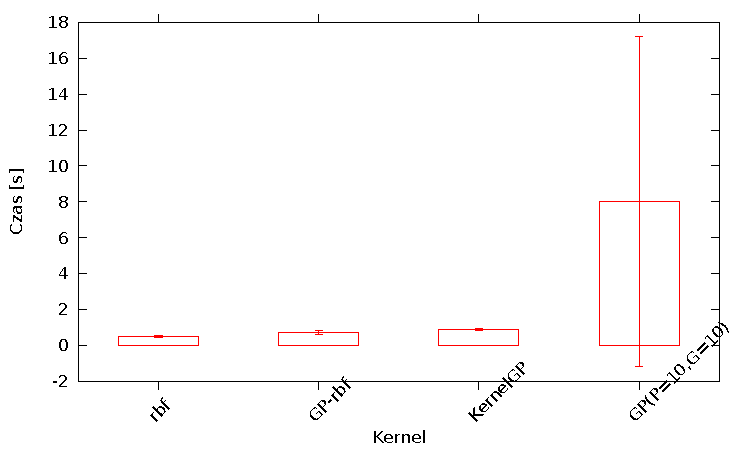
\includegraphics[scale=0.60]{figures/results/time/time-breast}
	\caption{Czasy uczenia i klasyfikacji zbioru breast dla różnych funkcji jądrowych i algorytmów. \label{fig:time-some-breast}}
\end{figure} 

\begin{figure}
	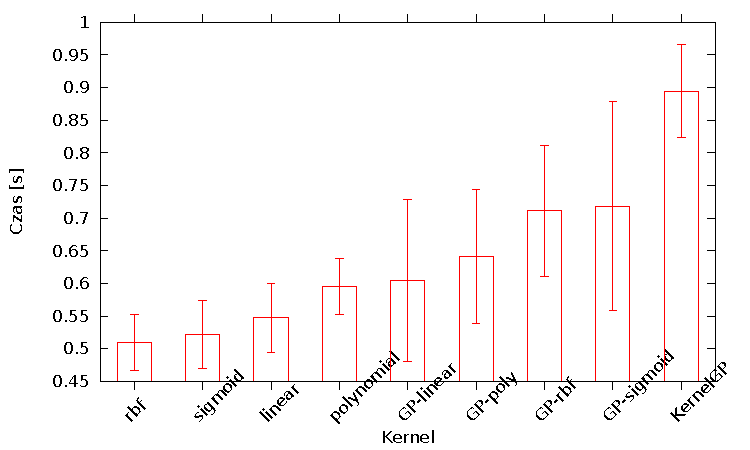
\includegraphics[scale=0.60]{figures/results/time/time_almost_all_breast}
	\caption{Czasy uczenia i klasyfikacji zbioru breast dla różnych funkcji jądrowych i algorytmów. \label{fig:time-all-breast}}
\end{figure} 



\section{Użycie pamięci}

\section{Posdumowanie wyników}

\clearpage
